\chapter[Metodologia]{Metodologia}

	De acordo com \cite{metodologiaCientifica}, a metodologia de pesquisa adotada neste trabalho pode ser classificada nas seguintes categorias: classificação quanto aos objetivos da pesquisa, quanto à natureza da pesquisa, quanto à escolha do objeto de estudo, quanto à técnica de coleta de dados, e quanto à técnica de análise de dados. A classificação escolhida em cada categoria busca garantir conhecimento amplo sobre diferentes técnicas de solução do problema de SLAM, possibilitando a adaptação de técnicas para um contexto de robôs simples. Nas seções seguintes, são apresentadas as categorias e suas respectivas classificações de pesquisa adotadas para este trabalho. 

	\section{Classificação da Pesquisa} % (fold)
	\label{sec:classificação_da_pesquisa}
		
		De acordo com \cite{metodologia}, uma pesquisa científica pode ser classificada nas categorias \textit{abordagem da pesquisa}, \textit{natureza da pesquisa}, \textit{objetivos da pesquisa}, e \textit{procedimentos}, que são apresentadas nas seções \ref{sub:abordagem_da_pesquisa}, \ref{sub:natureza_da_pesquisa}, \ref{sec:classificação_quanto_aos_objetivos_da_pesquisa} e \ref{sub:procedimentos}, respectivamente.



		\subsection{Abordagem da pesquisa} % (fold)
		\label{sub:abordagem_da_pesquisa}

			A classificação deste trabalho em relação à abordagem da pesquisa é definida como \textit{qualitativa}. Segundo \cite{metodologiaCientifica}, abordagens de cunho qualitativo buscam o significado dos dados obtidos, capturando, além da aparência do fenômeno estudado, suas essências. Dessa forma, a pesquisa qualitativa envolve a obtenção e a análise dos dados descritivos por meio do contato direto entre o pesquisador e o fenômeno estudado \cite{metodologiaCientifica}. 

			A abordagem qualitativa não busca definir resultados de maneira quantificável, como mostra \cite{metodologia}, buscando compreender de forma subjetiva o evento estudado. Nesse trabalho, os dados serão coletados em ambiente controlado e analisados de forma não quantificável, buscando caracterizar os resultados como, por exemplo, satisfatórios ou não, caracterizando, assim, segundo \cite{metodologia}, uma pesquisa qualitativa.

		Sua utilização, durante este trabalho, tem como objetivo, entender detalhadamente o funcionamento de diversas técnicas de resolução do problema de SLAM, viabilizando a adaptação das mesmas para um contexto limitado. Além disso, a proximidade do pesquisador com o fenômeno a ser estudado possibilita um análise descritiva dos dados de forma que viabilize uma adaptação de técnicas para contextos limitados.
		
		% subsection abordagem_da_pesquisa (end)

		\subsection{Natureza da pesquisa} % (fold)
		\label{sub:natureza_da_pesquisa}
		
			A classificação deste trabalaho em relação à natureza da pesquisa é definida como \textit{pesquisa aplicada}, devido ao fato de buscar solucionar um problema recorrente no contexto mundial da robótica. Segundo \cite{metodologia}, \textit{"a pesquisa aplicada busca gerar conhecimentos para aplicação prática, dirigidos à solução de problemas específicos"}.
		% subsection natureza_da_pesquisa (end)

		\subsection{Objetivos da pesquisa} % (fold)
		\label{sec:classificação_quanto_aos_objetivos_da_pesquisa}
			
			A classificação deste trabalho em relação aos objetivos da pesquisa é definida como \textit{exploratória}. De acordo com \cite{metodologiaCientifica}, a pesquisa exploratória tem como objetivo ampliar os conhecimentos do pesquisador sobre o tema. A pesquisa exploratória é, normalmente, o primeiro passo quando o pesquisador não conhece suficientemente a área que pretende abordar \cite{metodologiaDaPesquisa}.

			O uso da pesquisa exploratória, neste trabalho, se dá pela necessidade do conhecimento sobre as diversas técnicas de resolução do problema de SLAM, com o objetivo de possibilitar adaptações das mesmas para o contexto de robôs simples.
		% section classificação_quanto_aos_objetivos_da_pesquisa (end)

		\subsection{Procedimentos} % (fold)
		\label{sub:procedimentos}

			Quanto aos procedimentos da pesquisa, a mesma foi dividida em duas etapas. Durante a primeira etapa o procedimento seguido foi \textit{pesquisa bibliográfica}. A qual, segundo \cite{metodologia}, é feita a partir do levantamento de referências teóricas publicadas por meio de livros, artigos, paginas da web, entre outros.

			Já na segunda etapa do trabalho, o procedimento a ser seguido será o de \textit{pesquisa-ação}. Como \cite{metodologia} afirma, \textit{"a pesquisa-ação pressupõe uma participação planejada do pesquisador na situação problemática a ser investigada"}. Além da participação do pesquisador, o objeto de estudo da pesquisa-ação não pode ser representado por um conjunto de variáveis que poderiam ser analisadas separadamente \cite{metodologia}.

			A utilização da \textit{pesquisa-ação} durante este trabalho é devido ao conhecimento que será obtido pelo pesquisador durante a participação ativa na situação estudada, possibilitando análises amplas de todo o contexto.
		
		% subsection procedimentos (end)

	
	De acordo com a classificação da pesquisa nas diferentes categorias apresentadas acima, a tabela \ref{tab:metodologia} apresenta, de maneira resumida, a abordagem definida para realização deste trabalho.

	\begin{table}[H]
		\centering
		\caption{Classificação da pesquisa}
		\label{tab:metodologia}
		\begin{tabular}{|c|c|c|c|c|}
		\hline
		\textbf{\begin{tabular}[c]{@{}c@{}}Abordagem \\ da pesquisa\end{tabular}} & 
		\textbf{\begin{tabular}[c]{@{}c@{}}Natureza \\ da pesquisa\end{tabular}} & 
		\textbf{\begin{tabular}[c]{@{}c@{}}Objetivos \\ da pesquisa\end{tabular}} & 
		\textbf{Procedimentos} \\ \hline
		Qualitativa                                                              & Aplicada                                                              & \begin{tabular}[c]{@{}c@{}}Exploratória \end{tabular}      & \begin{tabular}[c]{@{}c@{}}Pesquisa bibliográfica/\\ Pesquisa-ação \end{tabular} \\ \hline
		\end{tabular}
	\end{table}

	De acordo com \cite{fundamentosMetodologia}, a partir da classificação da pesquisa, fica fácil estabelecer o \textit{caminho} a ser seguido para realização da mesma. Portanto, definiu-se o processo metodológico, o qual é apresentado na seção \ref{sec:processo_metodológico}.


\section{Processo Metodológico} % (fold)
\label{sec:processo_metodológico}

% section processo_metodológico (end)

O TCC, segundo as regras da UnB, é realizado em duas fases: uma chamada de TCC\_01 e outra chamada de TCC\_02. Durante o TCC\_01, o foco desse trabalho será estabelecer os pilares teóricos para embasamento do projeto como um todo, bem como desenvolver uma prova de conceito visando estudar a viabilidade da proposta. Já durante o TCC\_02, o trabalho estará focado em atingir o objetivo geral \textit{"Adaptar técnicas de resolução do problema de SLAM para o contexto de robôs simples, utilizando os kits de robótica Mindstorms da Lego, em um primeiro momento."}, com base nas fundamentações teóricas e nos resultados acordados na prova de conceito, ambos - fundamentações e resultados - conquistados ao longo do TCC\_01.

O TCC\_01 pôde ser sub-dividido em oito atividades: \textit{selecionar tema}, \textit{realizar pesquisa bibliográfica}, \textit{definir proposta}, \textit{escrever referencial teórico}, \textit{estabelecer suporte tecnológico}, \textit{evoluir metodologia}, \textit{realizar prova de conceito} e \textit{apresentar TCC 1}. As mesmas estão distribuídas de acordo com o cronograma disposto na tabela \ref{tab:cronograma}.

\begin{table}[H]
	\centering
	\begin{tabular}{|c|c|c|c|c|}
		\hline
		\textbf{Cronograma}             & \textbf{Março} & \textbf{Abril} & \textbf{Maio} & \textbf{Junho} \\ \hline
		Selecionar Tema                 & X              &                &               &                \\ \hline
		Realizar pesquisa bibliográfica & X              & X              & X             & X              \\ \hline
		Definir proposta                & X              &                &               &                \\ \hline
		Escrever referencial teórico    &                & X              & X             &                \\ \hline
		Estabelecer suporte tecnológico &                & X              & X             & X              \\ \hline
		Evoluir metodologia             &                & X              & X             &                \\ \hline
		Realizar prova de conceito      &                &                &               & X              \\ \hline
		Apresentar TCC 1                &                &                &               & X              \\ \hline
	\end{tabular}
	\caption{Cronograma TCC 1}
	\label{tab:cronograma}
\end{table}

Com o objetivo de definir e acompanhar o processo de desenvolvimento da primeira etapa do trabalho de conclusão de curso, foi modelado um processo metodológico, o qual se encontra na figura \ref{img:processo}.

\begin{figure}[H]
	\centering
	\caption{Processo Metodológico}
	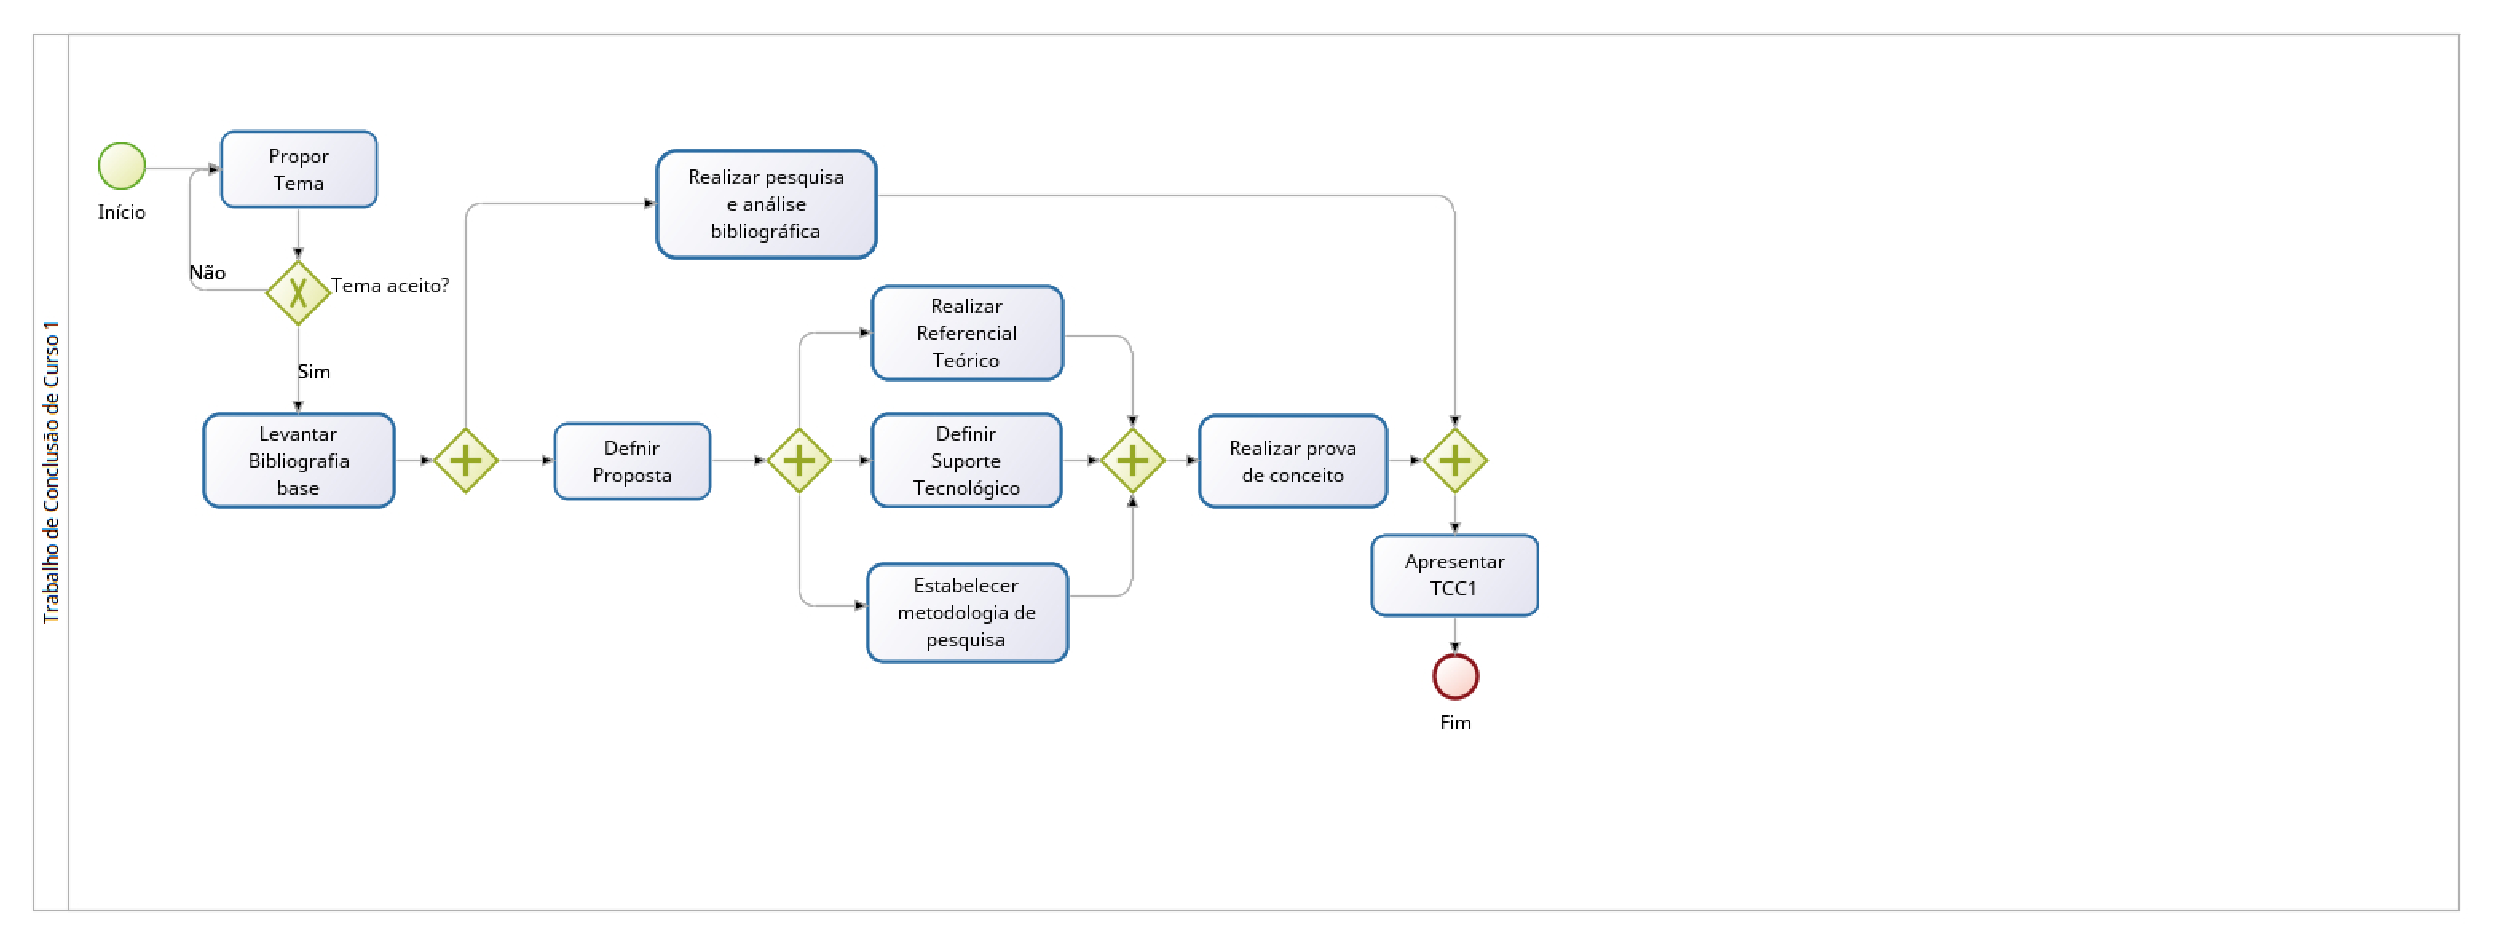
\includegraphics[scale=0.6]{figuras/processo.eps}
	\label{img:processo}
\end{figure}

\begin{itemize}
	\item \textbf{Propor tema}:

		A atividade de propor tema engloba desde a escolha do contexto em que se deseja trabalhar, até a definição dos orientadores do trabalho. Após a escolha do contexto e dos orientadores, buscou-se definir um escopo que será abordado durante o trabalho, ou seja, o tema. Os orientadores devem validar o tema escolhido para concluir a atividade.

	\item \textbf{Levantar bibliografia base}:

		Esta atividade refere-se à definição de pilares para o estudo proposto, ou seja, estabelecer o marco teórico do trabalho. Este levantamento garante o entendimento do contexto trabalhado e as possibilidades de atuação, especificando mais adequadamente o escopo.

	\item \textbf{Definir Proposta}:

		Documentar a proposta de pesquisa para este trabalho. A proposta inclui, não apenas, mas, principalmente, uma introdução com a contextualização do tema, o objetivo geral e específicos, a justificativa e uma metodologia de pesquisa.

	\item \textbf{Realizar pesquisa e análise bibliográfica}:

		A pesquisa bibliográfica foi feita a partir da utilização da técnica de \textit{revisão sistemática}, com o objetivo de ampliar os conhecimentos em relação ao tema, conhecendo pesquisas em diferentes contextos e de diversas bases científicas, como \textit{IEEE, Scopus, Springer} e \textit{CAPES}. O detalhamento da revisão sistemática encontra-se na seção \ref{sec:resultados_parciais}.

	\item \textbf{Realizar referencial teórico}:

		Trata-se da escrita do capítulo dois deste trabalho. O mesmo descreve o referencial teórico do trabalho em andamento. Como insumos para esta atividade, encontram-se todas as pesquisas bibliográficas obtidas durante a atividade de \textit{Realizar pesquisa e análise bibliográfica}. No segundo capítulo deste trabalho, o tema será especificado com mais detalhe.

	\item \textbf{Definir suporte tecnológico}:

		Nesta atividade, são definidas as principais ferramentas e tecnologias utilizadas para a execução deste trabalho. 

	\item \textbf{Estabelecer metodologia de pesquisa}:

		Durante esta atividade, a metodologia de pesquisa inicial, apresentada durante a \textit{proposta}, foi evoluída, com o objetivo de adequar as formas de atuação ao longo da realização do trabalho proposto. 

	\item \textbf{Realizar prova de conceito}:

		Durante esta atividade foi realizada a implementação de uma prova de conceito que buscou avaliar a viabilidade da realização deste trabalho. Durante a prova de conceito, que se encontra detalhada na seção \ref{sec:prova_conceito}, ferramentas e maneiras de mapear ambientes foram estudadas.

	\item \textbf{Apresentar TCC 1}:

		Apresentar os resultados obtidos até o momento para a banca examinadora.
\end{itemize}

As atividades de \textit{Levantar bibliografia base} e \textit{Realizar pesquisa e análise bibliográfica} foram desenvolvidas utilizando a técnica de revisão sistemática, a qual se encontra detalhada na seção \ref{sec:revisao_sistematica}.

\subsection{Revisão Sistemática} % (fold)
\label{sec:revisao_sistematica}

	Durante décadas, as pesquisas se encontravam carentes de métodos científicos que detalhassem o processo de revisão de literatura, como mostra \cite{revisao_sistematicaUfrj}. Esta carência acaba por impossibilitar a realização futura da mesma busca, já que sem detalhamento da pesquisa, o interessado não poderá aplicar a busca, realizando comparações, por exemplo. Desse modo, entre as décadas de 70 e 80, psicólogos e cientistas sociais buscaram definir métodos de sistematizar revisões de litetarura, as chamadas \textit{revisões sistemáticas}.  
	
	Com o objetivo de realizar uma ampla pesquisa bibliográfica, buscando conhecer diferentes técnicas de auto-localização e, mais especificamente, o problema de SLAM, utilizou-se da técnica de revisão sistemática. Uma revisão sistemática busca identificar e analisar o máximo de pesquisas relacionadas a um tema em específico, como define \cite[p. 8]{revisaoSistematicaComunicacao}:

	 \begin{quote}
	 	\textit{"Uma revisão literária sistemática é um meio de identificar, avaliar e interpretar
		todas as pesquisas disponíveis relevantes a uma determinada questão de pesquisa,
		ou área de um tópico, ou fenômeno de interesse. Estudos individuais que contribuem
		para uma revisão sistemática são chamados estudos primários; uma revisão
		sistemática é uma forma de estudo secundário."}
	 \end{quote}

	 Como afirma \cite{revisaoSistematicaComunicacao}, a técnica de revisão sistemática é bastante utilizada quando se busca identificar soluções propostas para resolver o problema levantado. Neste trabalho, a revisão sistemática busca identificar técnicas de resolução do problema de SLAM em diferentes contextos, inclusive educacional.

	 \subsubsection{Processo de Revisão Sistemática}

	 	O processo utilizado durante a pesquisa segue o processo de revisão sistemática apresentado por \cite{Kitchenham}. Desse modo, o processo é dividido em três etapas: \textit{planejamento da revisão}, \textit{condução da revisão} e a \textit{documentação da revisão}. As atividades que estão distribuídas entre essas etapas podem ser observadas na figura \ref{img:processo_revisao_sistematica}.

	 	\begin{figure}[H]
			\centering
			\caption{Processo de revisão sistemática. Processo adaptado de \cite{Kitchenham}}
			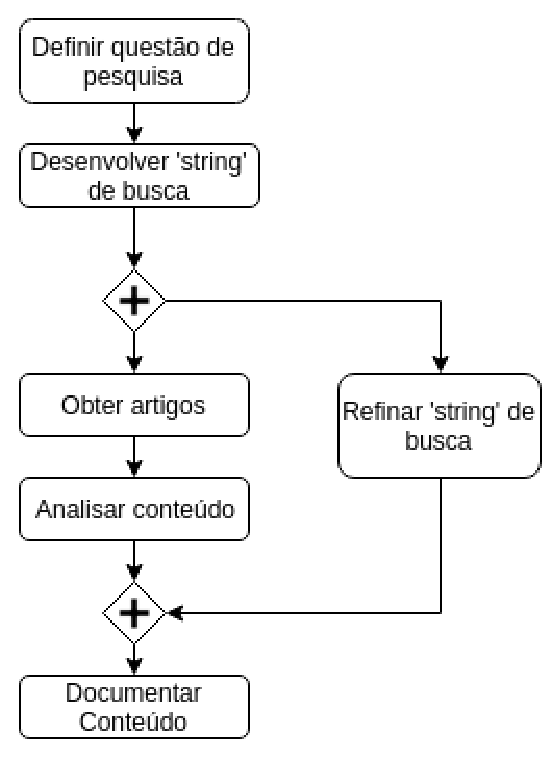
\includegraphics[scale=0.8]{figuras/processo_revisao_sistematica.eps}
			\label{img:processo_revisao_sistematica}
		\end{figure}

		A descrição de cada atividade do processo da figura \ref{img:processo_revisao_sistematica} encontra-se na tabela \ref{tab:descricaoAtividades}.

		\begin{table}[H]
			\centering
			\caption{Processo de revisão sistemática}
			\label{tab:descricaoAtividades}
			\begin{tabular}{|c|c|}
				\hline
				\rowcolor[HTML]{C0C0C0} 
				\textbf{Atividade}                                                                  & \textbf{Descrição}                                                                                                                                                                                                                                                                   \\ \hline
				\textbf{\begin{tabular}[c]{@{}c@{}}Definir questão \\ de pesquisa\end{tabular}}     & \begin{tabular}[c]{@{}c@{}}Atividade relacionada à definição do objetivo final da pesquisa,\\ o que o pesquisador deseja alcançar com a mesma. A\\ definição da questão de pesquisa possibilita o estabelecimento\\ de critérios de busca durante os ciclos de revisão.\end{tabular} \\ \hline
				\textbf{\begin{tabular}[c]{@{}c@{}}Desenvolver \\ \textit{string}\\ de busca\end{tabular}} & \begin{tabular}[c]{@{}c@{}}Atividade de desenvolvimento. Na qual o objetivo é definir uma \textit{string}\\ de busca que represente todo o trabalho pesquisado. A \textit{string} \\ será refinada ao longo de toda pesquisa, buscando maximizar a\\ efetividade das buscas.\end{tabular}               \\ \hline
				\textbf{Obter artigos}                                                              & \begin{tabular}[c]{@{}c@{}}A partir da definição de um critério de busca, os artigos que se \\ enquadram neste critério são selecionados para análise. A obtenção\\ deve ser realizada em diferentes bases científicas, como IEEE, Scopus,\\ Springer e CAPES.\end{tabular}          \\ \hline
				\textbf{\begin{tabular}[c]{@{}c@{}}Analisar \\ conteúdo\end{tabular}}               & \begin{tabular}[c]{@{}c@{}}A análise do conteúdo busca, além de estudar o tema pesquisado, \\ conhecer novas pesquisas e, com isso, refinar a \textit{string} de busca.\end{tabular}                                                                                                          \\ \hline
				\textbf{\begin{tabular}[c]{@{}c@{}}Refinar a \\ \textit{string} de busca\end{tabular}}     & \begin{tabular}[c]{@{}c@{}}Esta atividade é considerada uma das atividades mais importantes\\ do processo de revisão sistemática. Busca maximizar a efetividade\\ do processo de busca, identificando artigos importantes para a pesquisa.\end{tabular}                              \\ \hline
				\textbf{\begin{tabular}[c]{@{}c@{}}Documentar\\ conteúdo\end{tabular}}              & \begin{tabular}[c]{@{}c@{}}A documentação do conteúdo, basicamente, é definida como o registro\\ das informações necessárias à pesquisa, obtidas com os ciclos de pesquisa.\\ Os resultados da revisão sistemática são frutos desta atividade.\end{tabular}                          \\ \hline
			\end{tabular}
		\end{table}
	
	O detalhamento do desenvolvimento da revisão sistemática, como os ciclos de busca e o processo de refinamento da \textit{string} estão detalhados no capítulo \ref{sec:resultados_parciais}.
% section revisão_sistemática (end)
%Quanto aos procedimentos de desenvolvimento, durante a fase de adaptação de técnicas de resolução do problema de SLAM, a metodologia seguida será baseada no \textit{Scrum}, utilizando sprints de 2 semanas. O desenvolvimento se dará com base em provas de conceito que buscarão sustentar a viabilidade das adaptações propostas.
